\documentclass{article}[12pt]
\usepackage{verbatim}
\usepackage{graphicx}
\usepackage{latexsym}
\usepackage{amsmath}
\usepackage{qtree}
\usepackage{fullpage}

\title{CS240 Assignment 4}
\author{Nissan Pow}

\begin{document}
\maketitle

\section*{Question 1}
\subsection*{(a)}

\begin{tabular}{|c|c|c|c|}
  \hline
  Search & MTF & Transpose & MTM \\
  \hline
  3 & [0,1,2,3,4,5,6] & [0,1,2,3,4,5,6] & [0,1,2,3,4,5,6] \\
  1 & [3,0,1,2,4,5,6] & [0,1,3,2,4,5,6] & [0,1,2,3,4,5,6] \\
  6 & [1,3,0,2,4,5,6] & [1,0,3,2,4,5,6] & [0,2,3,1,4,5,6] \\
  5 & [6,1,3,0,2,4,5] & [1,0,3,2,4,6,5] & [0,2,3,6,1,4,5] \\
  5 & [5,6,1,3,0,2,4] & [1,0,3,2,4,5,6] & [0,2,3,5,6,1,4] \\
  2 & [5,6,1,3,0,2,4] & [1,0,3,2,5,4,6] & [0,2,3,5,6,1,4] \\
  4 & [2,5,6,1,3,0,4] & [1,0,2,3,5,4,6] & [0,3,5,2,6,1,4] \\
  \ & [4,2,5,6,1,3,0] & [1,0,2,3,4,5,6] & [0,3,5,4,2,6,1] \\
  \hline
\end{tabular}

\subsection*{(b)}

Use the following array to answer questions a and b.

\begin{tabular}{|c|p{3.2cm}|p{3.2cm}|p{3.2cm}|}
\hline
Search & MTF & Transpose & MTM\\
\hline
\hline
Start&
\multicolumn{3}{|c|}{\tt [0,1,2,3,4,5,6]}\\
\hline
\hline
3&
&
&
\\
&
c=4 \hspace{.5cm}, m=5 \hspace{.5cm} &
c=4 \hspace{.5cm}, m=3 \hspace{.5cm} &
c=4 \hspace{.5cm}, m=0 \hspace{.5cm} \\
\hline
1&
&
&
\\
&
c=3 \hspace{.5cm}, m=4 \hspace{.5cm} &
c=2 \hspace{.5cm}, m=3 \hspace{.5cm} &
c=2 \hspace{.5cm}, m=4 \hspace{.5cm} \\
\hline
6&
&
&
\\
&
c=7 \hspace{.5cm}, m=8 \hspace{.5cm} &
c=7 \hspace{.5cm}, m=3 \hspace{.5cm} &
c=7 \hspace{.5cm}, m=5 \hspace{.5cm} \\
\hline
5&
&
&
\\
&
c=7 \hspace{.5cm}, m=8 \hspace{.5cm} &
c=7 \hspace{.5cm}, m=3 \hspace{.5cm} &
c=7 \hspace{.5cm}, m=5 \hspace{.5cm} \\
\hline
5&
&
&
\\
&
c=1 \hspace{.5cm}, m=0 \hspace{.5cm} &
c=6 \hspace{.5cm}, m=3 \hspace{.5cm} &
c=4 \hspace{.5cm}, m=0 \hspace{.5cm} \\
\hline
2&
&
&
\\
&
c=6 \hspace{.5cm}, m=7 \hspace{.5cm} &
c=4 \hspace{.5cm}, m=3 \hspace{.5cm} &
c=2 \hspace{.5cm}, m=4 \hspace{.5cm} \\
\hline
4&
&
&
\\
&
c=7 \hspace{.5cm}, m=8 \hspace{.5cm} &
c=6 \hspace{.5cm}, m=3 \hspace{.5cm} &
c=7 \hspace{.5cm}, m=5 \hspace{.5cm} \\
\hline
\hline
\hline
Total comparisons&
35  & 36 & 33 \\
\hline
Total movements&
40  & 21 & 23 \\
\hline
\end{tabular}

\subsection*{(c)}
Since MTF, Transpose, and MTM are all within a constant factor of $C_{OPT}$ (MTF $< 2C_{OPT}$ from slides), the asymptotic order of the average performance of each of those heuristics is $O(1)$.

\section*{Question 2}
Use a data structure that's a hybrid between a BTree and a Heap, which I shall call BHeap. A BHeap of order $d$ is a Heap such that: \\
\begin{itemize}
  \item every node has $\le d$ children
  \item every non-root node has $\ge \lceil \frac{d}{2} \rceil$ children
  \item all external nodes have the same depth
  \item every node itself is structured as a Heap
\end{itemize}

Choose $d$ such that one $d$-node fills exactly one disk page. Thus the height of the BHeap will be $O(\log_{B}n)$.
Basically to SiftUp/SiftDown, we retrieve a ``node'' (which is actually a heap), perform the usual SiftUp/SiftDown on this node, and continue retrieving nodes and sifting up/down if necessary. This will require $O(\log_{B}n)$ disk accesses. Hence, ExtractMin and Insert each use at most $O(\log_{B}n)$ disk accesses.

\section*{Question 3}
\subsection*{(a)}

\begin{tabular}{r|c|c|c|c|c|c|c|}
    & Insert 31 & Insert 26 & Insert 16 & Insert 23 & Insert 11 & Insert 30 & Insert 20 \\
\hline
0:  &           &           &           &           &           & 30        & 20        \\
\hline
1:  & 31        & 31        & 31        & 31        & 11        & 11        & 11        \\
\hline
2:  &           &           &           &           & 31        & 31        & 30        \\
\hline
3:  &           &           &           & 23        & 23        & 23        & 23        \\
\hline
4:  &           &           &           &           &           &           & 31        \\
\hline
5:  &           &           &           &           &           &           &           \\
\hline
6:  &           & 26        & 16        & 16        & 16        & 16        & 16        \\
\hline
7:  &           &           & 26        & 26        & 26        & 26        & 26        \\
\hline
8:  &           &           &           &           &           &           &           \\
\hline
9:  &           &           &           &           &           &           &           \\
\hline
\end{tabular}

\subsection*{(b)}
When inserting any key $k$, if we encounter a key $k'$ with $k'>k$, we swap to put $k$ in this position and then proceed to insert $k'$.
This ensures that for all keys with the same value of $f(x)$, the keys encountered before it in its probe sequence are all smaller than it.
Now consider any arbitrary probe sequence with last value $x$; by the argument above, $x$ is the largest value in its probe sequence.
Now suppose another key, $y$, with $y>x$ and $f(x) \neq f(y)$, is supposed to be inserted in the middle of this probe sequence. Since
we are doing linear probing, there cannot be any empty spaces in $x$'s probe sequence. Therefore $y$ has to be probed as well. And since
$y>x$, $y$ will be inserted \emph{after} the end of $x$'s probe sequence, thus maintaining the assertion above. Hence for any key, the keys encountered before it in its probe sequence are all smaller than it.

\subsection*{(c)}
When searching for an element,$x$, that's not present in the hash, if we encounter an element that's greater than $x$ \emph{before} finding $x$, we can immediately terminate the search. This holds because of part (b) above. In the best case (or even average case), it improves the runtime of searches for elements not in the hash since we are able to terminate the search without probing the entire probe sequence.

\section*{Question 4}
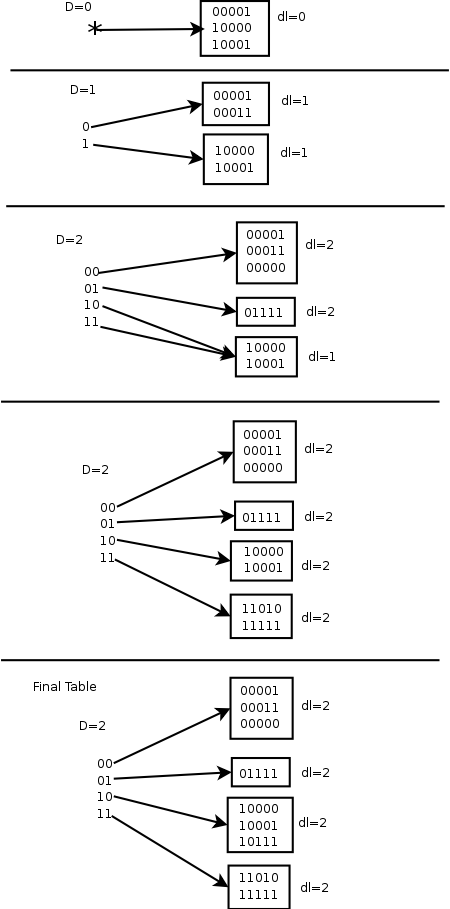
\includegraphics[scale=0.4]{a4q4.png}
\end{document}
